\documentclass[11pt,a4paper]{article}
\usepackage[utf8]{inputenc}
\usepackage{lmodern} % Must precede fontenc: the EC fonts may not be installed
\usepackage[T1]{fontenc}
\usepackage[margin=2.5cm]{geometry}
\usepackage{amsmath}
\usepackage{graphicx}
\usepackage{booktabs}
\usepackage{caption}

% Polish hyphenation is optional, so the report also compiles on TeX installations without it.
\IfFileExists{polish.ldf}{%
  \usepackage[polish]{babel}%
}{%
  \hyphenpenalty=10000
  \exhyphenpenalty=10000
  \emergencystretch=3em
  \renewcommand{\figurename}{Rysunek}
  \renewcommand{\tablename}{Tabela}
}

\title{Biosygnały, laboratorium 3--4:\\analiza HRV w dziedzinie częstotliwości}
\author{Dominik Zawlocki}
\date{5 listopada 2026}

\begin{document}
\maketitle

\section{Cel i dane}
Celem ćwiczenia było zaimplementowanie estymacji widma sygnałów próbkowanych niejednorodnie i~wyznaczenie parametrów HRV dla dwóch rzeczywistych zapisów odstępów RR:
\begin{itemize}
  \item \textbf{nsr001}: osoba zdrowa, rytm zatokowy, 106\,460 odstępów RR, 22,5~h zapisu,
  \item \textbf{chf206}: pacjent z~niewydolnością serca (NYHA~III), 135\,470 odstępów RR, 20,9~h zapisu.
\end{itemize}
Czasy załamków R wyznaczono jako sumę skumulowaną odstępów RR. Następnie odrzucono odstępy spoza zakresu 0,3--2~s (HR 30--200~bpm): 3 dla nsr001 i~28 dla chf206. Sumę liczono przed filtracją, aby usunięcie odstępu nie przesuwało kolejnych załamków na osi czasu.

\section{Metody}
Periodogram klasyczny i~periodogram Lomba--Scargle'a dane są wzorami:
\begin{gather}
P(f) = \frac{1}{N}\left[\Big(\sum_n x_n \cos(2\pi f t_n)\Big)^2 + \Big(\sum_n x_n \sin(2\pi f t_n)\Big)^2\right], \\
P_{LS}(f) = \frac{1}{2}\left\{\frac{\big(\sum_n x_n \cos(2\pi f [t_n-\tau])\big)^2}{\sum_n \cos^2(2\pi f [t_n-\tau])} + \frac{\big(\sum_n x_n \sin(2\pi f [t_n-\tau])\big)^2}{\sum_n \sin^2(2\pi f [t_n-\tau])}\right\}, \\
\tau = \frac{1}{4\pi f}\arctan\frac{\sum_n \sin(4\pi f t_n)}{\sum_n \cos(4\pi f t_n)}.
\end{gather}
W metodzie interpolacyjnej tachogram przepróbkowano do równomiernej siatki 4~Hz (najbliższy sąsiad, interpolacja liniowa, spline sześcienny) i~obliczono $P(f)$. W metodzie Lomba--Scargle'a korzystano bezpośrednio z~prawdziwych czasów uderzeń. W obu przypadkach od sygnału odjęto wartość średnią.

Periodogram przeliczono na jednostronną gęstość widmową mocy: $\mathrm{PSD} = 2P/f_s \cdot 10^6$ [ms$^2$/Hz], gdzie $f_s$ to 4~Hz po interpolacji lub średnia częstość uderzeń dla danych niejednorodnych. Przy takim skalowaniu pole pod PSD odpowiada wariancji sygnału. Parametry HRV wyznacza funkcja \texttt{compute\_hrv\_frequency\_metrics} (plik \texttt{hrv\_frequency.py}), która sumuje PSD w~pasmach Task Force (1996): ULF ${<}\,$0,003~Hz, VLF 0,003--0,04~Hz, LF 0,04--0,15~Hz, HF 0,15--0,4~Hz, przy kroku siatki częstotliwości $1/T$. Moc całkowita to $\mathrm{TP} = \mathrm{ULF}+\mathrm{VLF}+\mathrm{LF}+\mathrm{HF}$.

\section{Walidacja na sygnale syntetycznym}
Wygenerowano sinusoidę 0,1~Hz o~128 próbkach rozmieszczonych niejednorodnie. Wszystkie metody wskazują dominującą częstotliwość 0,1~Hz (rys.~\ref{fig:synth}). Na danych oryginalnych widoczne jest rozproszone tło w~całym zakresie częstotliwości, którego nie ma po interpolacji.

Dodatkowo sprawdzono skalowanie mocy na sinusoidzie 0,1~Hz o~amplitudzie 0,1~s, próbkowanej w~chwilach 3000 uderzeń. Oczekiwana moc to 5000~ms$^2$, a~w~paśmie LF uzyskano od 4741 do 4958~ms$^2$, zależnie od metody.

\begin{figure}[ht]
  \centering
  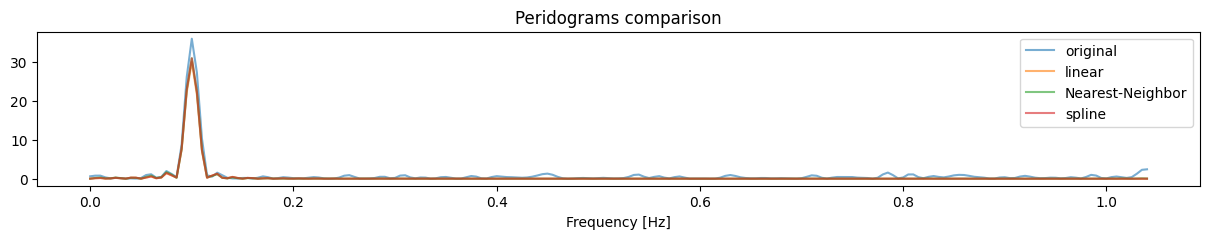
\includegraphics[width=\textwidth]{figures/synth_classic.png}\\[2mm]
  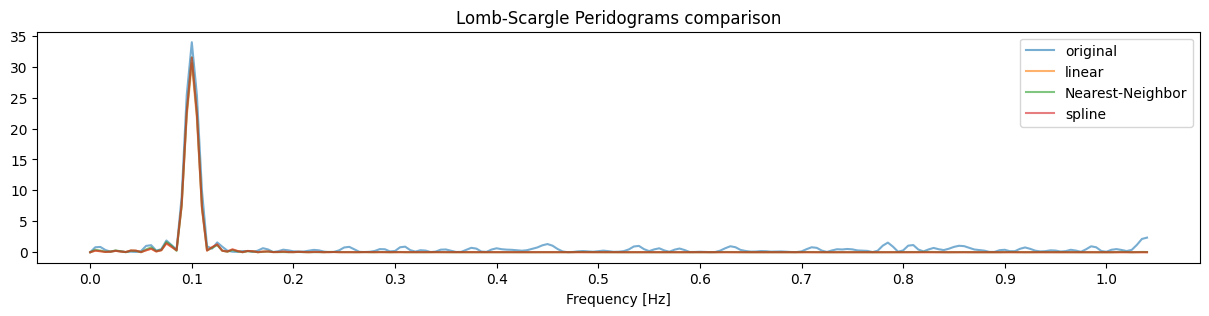
\includegraphics[width=\textwidth]{figures/synth_ls.png}
  \caption{Sygnał syntetyczny: periodogram klasyczny (u~góry) i~Lomba--Scargle'a (na dole), dla danych oryginalnych i~po interpolacji.}
  \label{fig:synth}
\end{figure}

\section{Wyniki dla sygnałów rzeczywistych}
Parametry HRV zebrano w~tab.~\ref{tab:hrv}, a~widma pokazano na rys.~\ref{fig:psd-nsr} i~\ref{fig:psd-chf}. Wykresy pochodzą z~notebooka \texttt{HRV.ipynb}, gdzie użyto rzadszej siatki (0,001--0,5~Hz, 1000 punktów), a~pasmo ULF nie jest na nich zaznaczone. Liczby w~tabeli pochodzą z~\texttt{hrv\_frequency.py}. Na siatce z~notebooka periodogram klasyczny policzony wprost na danych niejednorodnych dał praktycznie te same moce pasm co metoda Lomba--Scargle'a.

\begin{table}[ht]
  \centering
  \caption{Parametry HRV w~dziedzinie częstotliwości (moce w~ms$^2$).}
  \label{tab:hrv}
  \begin{tabular}{llrrrrrr}
    \toprule
    Sygnał & Metoda & ULF & VLF & LF & HF & TP & LF/HF \\
    \midrule
    nsr001 & Lomb--Scargle  & 24471 & 1983 & 510 & 253 & 27218 & 2,01 \\
           & najbliższy sąsiad & 27651 & 2194 & 715 & 428 & 30988 & 1,67 \\
           & liniowa        & 27654 & 2191 & 700 & 350 & 30895 & 2,00 \\
           & spline         & 27698 & 2199 & 731 & 488 & 31117 & 1,50 \\
    \midrule
    chf206 & Lomb--Scargle  & 1660 & 138 & 93 & 198 & 2089 & 0,47 \\
           & najbliższy sąsiad & 1251 & 155 & 233 & 393 & 2033 & 0,59 \\
           & liniowa        & 1251 & 153 & 218 & 292 & 1915 & 0,75 \\
           & spline         & 1258 & 248 & 369 & 548 & 2424 & 0,67 \\
    \bottomrule
  \end{tabular}
\end{table}

\begin{figure}[p]
  \centering
  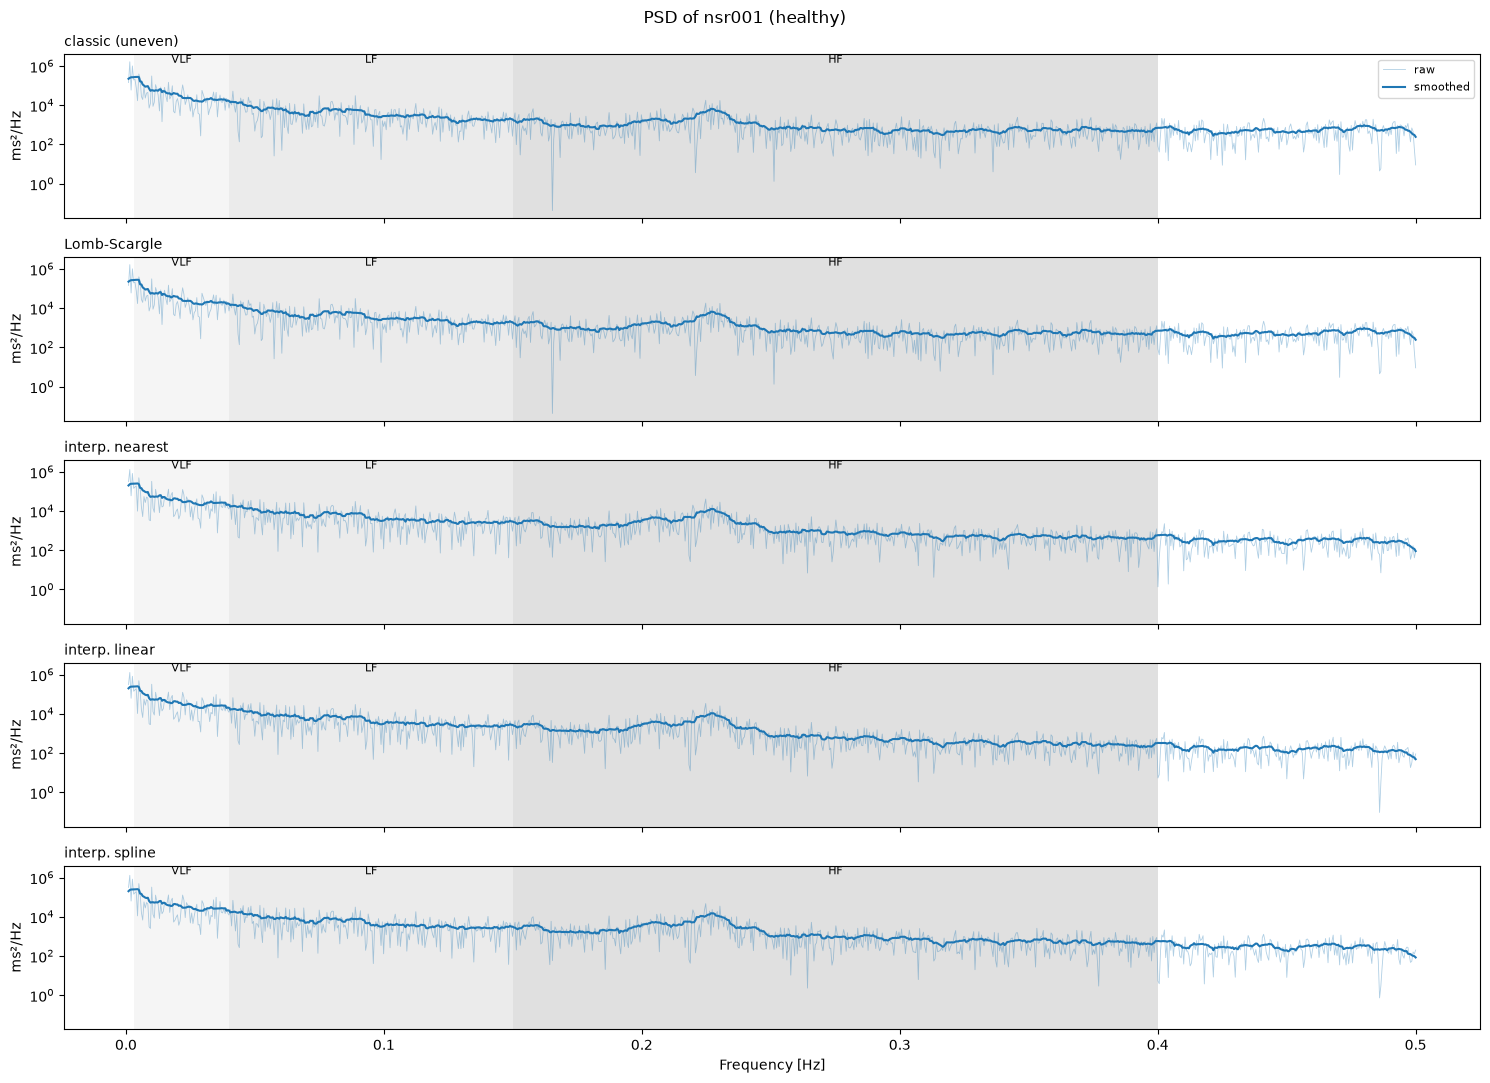
\includegraphics[width=0.9\textwidth]{figures/psd_nsr001.png}
  \caption{PSD sygnału nsr001. Widoczny jest pik oddechowy przy około 0,23~Hz.}
  \label{fig:psd-nsr}

  \vspace{4mm}
  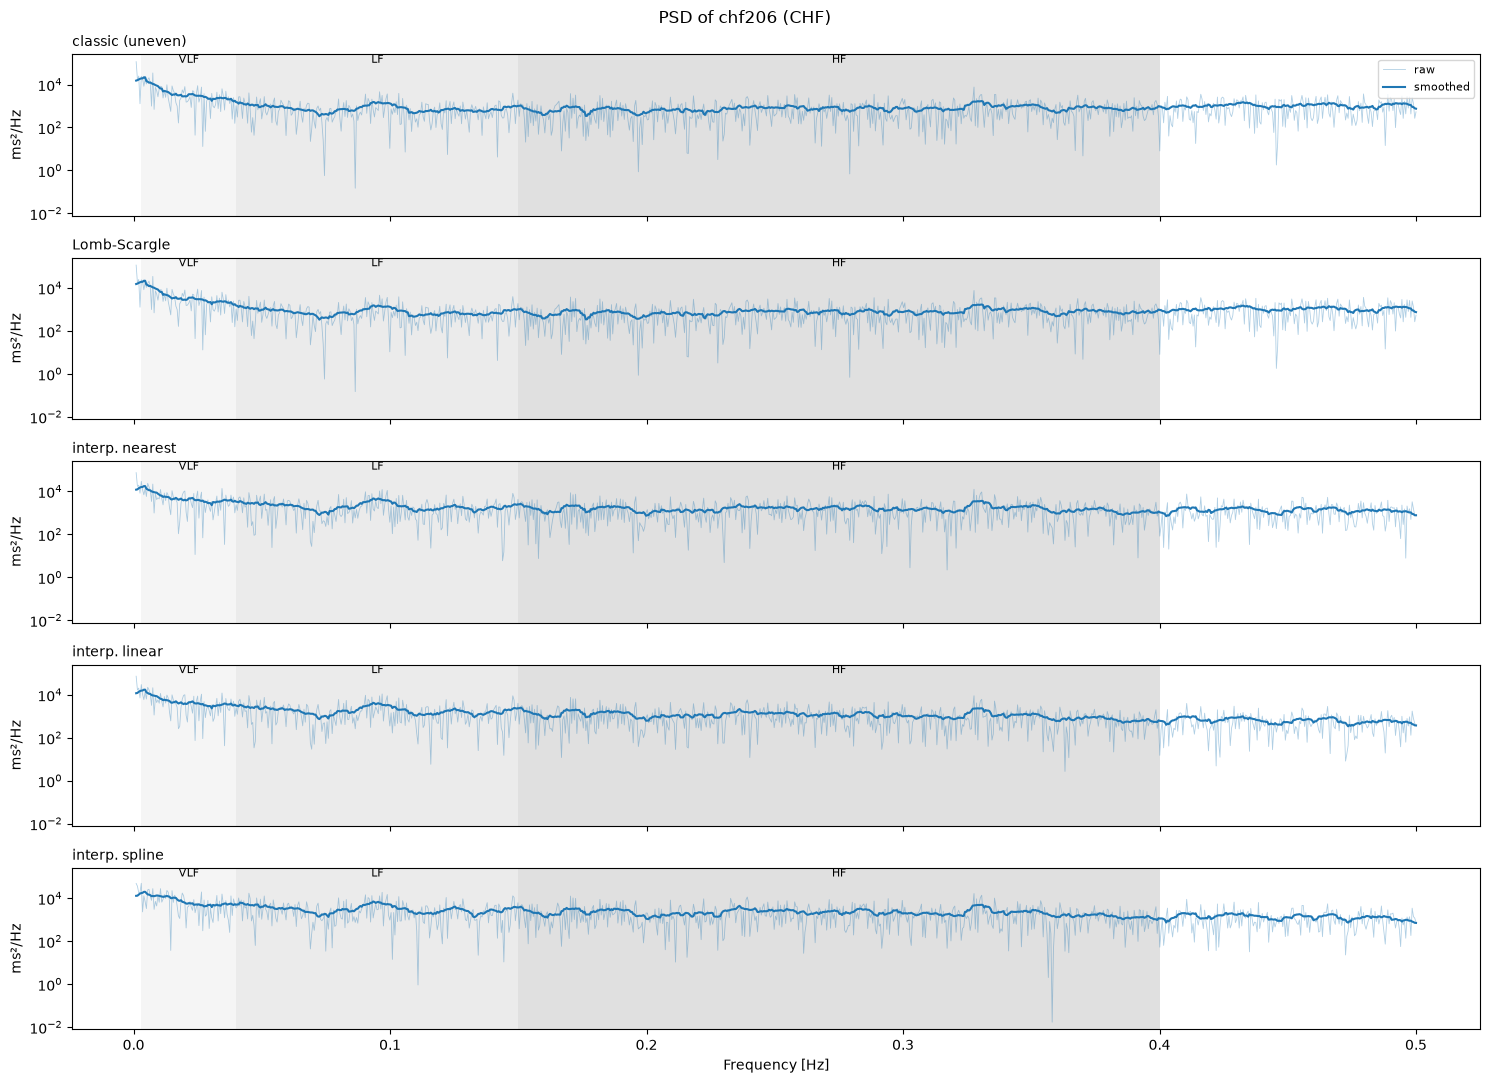
\includegraphics[width=0.9\textwidth]{figures/psd_chf206.png}
  \caption{PSD sygnału chf206. Powyżej około 0,05~Hz widmo jest niemal płaskie, bez wyraźnego piku oddechowego.}
  \label{fig:psd-chf}
\end{figure}

\section{Interpretacja}
\paragraph{Porównanie metod.} Interpolacja zawyża moc w~paśmie HF względem metody Lomba--Scargle'a: spline najbardziej (1,9-krotnie dla nsr001, 2,8-krotnie dla chf206), interpolacja liniowa najmniej (1,4 i~1,5-krotnie). W~paśmie LF efekt jest wyraźnie silniejszy dla chf206 (2,3--4,0-krotnie) niż dla nsr001 (1,4-krotnie). Mogą się do tego przyczyniać nieregularne uderzenia, ponieważ odfiltrowano tylko odstępy niefizjologiczne, a~nie pobudzenia ektopowe.

Na ULF i~TP wpływa też sposób ważenia danych. Lomb--Scargle traktuje każde uderzenie jednakowo, a~siatka równomierna waży równo czas. Wariancja RR zmienia się po interpolacji liniowej z~28\,442 do 30\,936~ms$^2$ dla nsr001 i~z~2317 do 2097~ms$^2$ dla chf206. Dlatego ULF po interpolacji jest dla nsr001 większe, a~dla chf206 mniejsze niż w~metodzie Lomba--Scargle'a.

\paragraph{Sygnał zdrowy a patologiczny.} Poniższe porównanie dotyczy wyników metody Lomba--Scargle'a.
\begin{itemize}
  \item \textbf{Całkowita zmienność:} TP jest u~pacjenta z~CHF około 13-krotnie mniejsze. Silne obniżenie HRV jest typowe dla niewydolności serca. Średnia częstość rytmu jest też wyższa (108 wobec 79~bpm).
  \item \textbf{ULF i~VLF:} obie moce są około 14-krotnie mniejsze, co oznacza znacznie słabszą zmienność wolnozmienną. ULF stanowi 90\% TP dla nsr001 i~79\% dla chf206, więc to ono dominuje w~TP przy zapisach wielogodzinnych.
  \item \textbf{LF:} moc spada około 5,5-krotnie (510 do 93~ms$^2$), co jest zgodne z~osłabieniem modulacji baroreceptorowej w~zaawansowanej CHF.
  \item \textbf{HF:} moc jest podobna (253 i~198~ms$^2$), ale ma inny charakter. Dla nsr001 w~widmie widać pik oddechowy, a~dla chf206 jest ono płaskie. Moc HF w~chf206 nie musi więc wynikać z~niemiarowości oddechowej i~może częściowo pochodzić od nieregularnych uderzeń.
  \item \textbf{LF/HF:} stosunek spada z~2,01 do 0,47. Ze względu na charakter pasma HF w~chf206 nie należy traktować tej wartości jako prostej miary równowagi współczulno-przywspółczulnej.
\end{itemize}

\section{Wnioski}
Metoda Lomba--Scargle'a działa bezpośrednio na prawdziwych czasach uderzeń, a~wyniki metody interpolacyjnej zależą od wybranego wariantu, szczególnie dla sygnału nieregularnego. Zapis chf206 wykazuje znacznie mniejszą zmienność rytmu niż nsr001, zwłaszcza w~pasmach ULF, VLF i~LF.

Ograniczenia: porównano tylko po jednym zapisie, od osób w~różnym wieku (64 i~38 lat), więc różnic nie można uogólniać ani przypisywać wyłącznie chorobie. Widma obejmują wielogodzinne zapisy łączące dzień i~noc, a~pobudzenia ektopowe nie zostały usunięte.

\end{document}
